\documentclass[man,floatsintext]{apa6}
\usepackage[nodoi]{apacite}
\usepackage{graphicx}
\usepackage[american]{babel}
\usepackage{amsmath}
\usepackage{enumitem}
\usepackage[section]{placeins}
\usepackage{caption}
\usepackage{subcaption}

\title{Preschoolers flexibly adapt to linguistic input in a noisy channel}
\author{Daniel Yurovsky, Sarah Case, and Michael C. Frank}
\affiliation{Stanford University}
\shorttitle{Noisy Channel Processing in Children}
\leftheader{Yurovsky \& Frank}


\abstract{
% When we process a speaker's utterance, we use more than the information in the speech signal. 
Because linguistic communication is inherently noisy and uncertain, adult language comprehenders integrate bottom-up cues from speech perception with top-down expectations about what speakers are likely to say. Further, in line with the predictions of ideal observer models, comprehenders flexibly adapt how much they rely on these two kinds of cues in proportion to their changing reliability. Do children also show evidence of flexible, expectation-based language comprehension? We presented 4- and 5-year-old children with ambiguous utterances that afforded two different interpretations, depending on whether they privileged perceptual input or linguistic expectations. Across two experiments, we manipulated the reliability of both their perceptual input and their expectations about the speaker's intended meaning. As predicted by noisy channel models of speech processing, children flexibly adjusted their interpretations as cues changed in reliability.}

\keywords{Language processing, noisy channel, cognitive development}

\authornote{Please address correspondence to: 

\vspace{12 pt}
Daniel Yurovsky

Jordan Hall (Building 420)

Stanford University

450 Serra Mall

Stanford, CA 94305

\vspace{12 pt}
Email: yurovsky@stanford.edu 

\vspace{24 pt}}

\begin{document}
\maketitle

Imagine Bob hears Alice say ``I had carrots and bees for dinner.'' Perhaps she visited an exotic restaurant, and he should ask how they tasted. Or perhaps he misheard her or she misspoke---she actually ate \emph{peas}. To interpret Alice's utterance, Bob has to integrate perceptual information from her speech with his expectations about what words usually go with ``carrots'' and ``dinner'' and what foods people usually eat. Modern statistical language processing systems use a body of theory based on this idea---that language is a \emph{noisy channel}, and that Bob can correct for perceptual errors using linguistic expectations about what Alice was likely trying to say \cite{jelinek1976, shannon1948}. 

Noisy channel principles provide a powerful framework for explaining how people process language in complex and uncertain real-time communicative situations \cite{clayards2008, levy2008, jaeger2010, kleinschmidt2015}. On this view of language, comprehenders integrate prior expectations with perceptual data; and they do so probabilistically, weighting each according to its reliability \cite{ernst2002, jacobs1999}. In one demonstration of such integration, \citeA{gibson2013} presented participants with semantically implausible sentences (e.g., ``The mother gave the candle the daughter''), which could have been produced by small typographical errors in otherwise much more plausible sentences (``The mother gave the candle \emph{to} the daughter''). Adult comprehenders were able to correct these errors, and critically corrected them more often when they thought the communicative channel was noisy (and hence the perceptual signal was unreliable). Conversely, adults corrected these errors less often when they thought they were in a ``silly'' context where many other sentences were similarly implausible. These results suggested that adults flexibly weigh information from the perceptual signal and from speaker expectations.

Do children also process language in the same flexible, expectation-based way? We know that children use speakers' social and pragmatic cues to determine their intended referent in otherwise ambiguous situations \cite{carpenter1998, clark2009}. We also know that children  use acoustic cues like speaker identity and linguistic cues like grammatical gender \cite{lew-williams2007, creel2012}. However, these successes have been shown only when all cues point to the same meaning, not when they disagree. In fact, children sometimes show striking deficits in revising incorrect expectations about meaning in cases where syntax and context compete \cite{trueswell1999}. But because these failures occur in complex contexts designed to test the development of other abilities, the question remains unanswered. Our current experiments test adaptive, expectation-based integration in the absence of other processing demands. 

We created a paradigm to independently manipulate expectations about speaker plausibility and perceptual noise. We introduced preschoolers (and, as a control group, adults) to either a Plausible or Implausible Speaker who initially uttered unambiguously different sentences like ``my cat has three little [kittens/hammers]'' (Figure \ref{fig:exposure}). Participants were then asked to resolve the intended meaning for ambiguous sentences like the ``bees/peas'' example above, which could either be the product of a perceptual error, or could convey implausible content (Figure \ref{fig:test}). If children integrate speaker expectations and channel noise, their interpretations should be a product of both. In Experiment 1, we first test this hypothesis by manipulating speaker plausibility. In Experiment 2, we replicate Experiment 1, and cross speaker plausibility with a manipulation of channel noise. The results of these experiments show that children, like adults, flexibly trade off between information sources in language comprehension in response to their reliability.

\begin{figure}[tb]
     \centering
        \begin{subfigure}[b]{.4 \textwidth}
            \caption{\label{fig:exposure}}
            
\includegraphics[width=\textwidth]{figures/exposure.pdf}
        \end{subfigure}\quad
        \vspace{12 pt}
        \begin{subfigure}[b]{.4 \textwidth}
           \caption{\label{fig:test}}
           
\includegraphics[width=\textwidth]{figures/testing.pdf}
        \end{subfigure}
    \caption{Example Exposure and Test trials. On Exposure trials, the two pictures and their corresponding referring expressions were highly distinct (e.g. ``my cat has three little [kittens/hammers].'' In contrast, the two pictures on Test trials could be referred to by expressions that contained a single phonological error (e.g. ``I had carrots and [bees/peas] for dinner.'' Children and adults introduced to a speaker who consistently referred to the plausible referent on Exposure were more likely to interpret a reference to the implausible picture on Test trials (``bees'') as a reference to the plausible picture (``peas'').}
   \label{fig:stimuli}
\end{figure}

\section{Experiment 1}

\subsection{Method}
\subsubsection{Participants}

Children were recruited at the Bing Nursery School on Stanford's campus. Each child was asked if they would be willing to play a game with the experimenter, and informed that they could stop playing at any time. Children were randomly assigned to speaker conditions, and we collected data until there were at least 20 participants in each condition (similar to other psycholinguistic studies of children \citeNP<e.g.>{trueswell1999, creel2012}). Data from a total of 43 children were collected; children were all between 4 and 6 years old, and approximately half were female. Neither age nor sex distribution varied significantly across conditions (Plausible: 23 children (12 girls), Mean age = 4.6 years (range = 4.0--5.3 years), Implausible: 20 children (10 girls), Mean age = 4.7 years (range = 4.1--5.4 years)).

Adult participants were recruited through Amazon Mechanical Turk. We posted 50 Human Intelligence Tasks (HITs) to be completed only by participants with US IP addresses that each paid 30 cents. A total of 50 HITs were posted, with Speaker condition assigned randomly to each participant. Fifty was chosen on the basis of the effect size in the child data.

\subsubsection{Stimuli, Design, and Procedure}

Experiment 1 consisted of a series of trials on which participants saw two pictures and heard a sentence referring to one of them. Pictures were constructed from clipart freely available on the internet, and audio was recorded by a female native speaker of English. In order to increase the ambiguity of the spoken utterances, and thus give us more power to detect error-correction, all of the audio recordings were convolved with a small amount of Brown noise.

Each trial contained one semantically plausible picture and one semantically implausible picture. On Exposure trials, these pictures and their corresponding referring expressions were highly distinct (Figure~\ref{fig:exposure}). In contrast, on Test trials the two pictures corresponded to referring expressions that were only one consonant or vowel apart (Figure~\ref{fig:test}). Each participant saw eight Exposure trials, followed by seven Test trials. The order of these trials within each of these two blocks was randomized across participants, as was the on-screen position of the two pictures on each trial. For participants in the Plausible Speaker condition, the speaker referred to the plausible referent on each of the eight Exposure trials. In contrast, for participants in the Implausible Speaker condition, the speaker referred to the implausible referent on each Exposure trial. In both conditions, the speaker referred to the implausible referent on all seven Test trials.

For all participants, the experiment began with a short introduction to Katie, the speaker who would be referring to pictures for the remainder of the task. After this introduction, participants completed the remaining trials, responding either with the mouse (adults), or by touching one of the pictures on an iPad (children). Adults were instructed by a series of written prompts; children were given instructions by a live experimenter. Three children's responses were coded from video due to a software error. All stimuli, data, and analyses are available at \small{\tt{http://github.com/dyurovsky/noisy-kids}}.

\subsection{Results}

In order to validate our manipulation, we first analyze the effect of the speaker on Exposure trials. If participants were attending to the speaker's requests during Exposure trials, those in the Plausible condition should have chosen the plausible referent (e.g. kittens) and those in the Implausible condition should have chosen the implausible referent (e.g. hammers). We provide two convergent analysis that show that they did. 

First, we asked whether participants selected the correct referent in each condition at levels different from chance. We submitted performance for each age group and condition separately to a mixed-effects logistic regression with random effects of subject and trial. Both children and adults were significantly more likely than chance to choose the plausible referent in the Plausible condition ($\beta_{adult} = 5.66$, $z = 6.76$, $p <.001$; $\beta_{child} = 2.62$, $z = 5.43$, $p <.001$), and significantly less likely than chance to choose the plausible referent in the Implausible condition ($\beta_{adult} = -3.87$, $z = -7.13$, $p <.001$; $\beta_{child} = -1.9$, $z = -5.61$, $p <.001$). Second, we compared performance across conditions, fitting a mixed-effects regression predicting choice on Exposure trials from age group, condition, and their interaction, and found significant effects of all three ($\beta_{child} = 1.96$,  $z = 3.33$, $p <.001$, $\beta_{Plausible Speaker} = 9.52$,  $z = 7.87$, $p <.001$,  $\beta_{child\: \cdot \: Plausible Speaker} = -5$,  $z = -4.12$, $p <.001$). Thus, both children and adults were sensitive to the speaker manipulation during Exposure trials, selecting the appropriate referent whether or not the request was implausible (although adults selected the correct referent more often in both conditions).

\begin{figure}[t]
\centering
     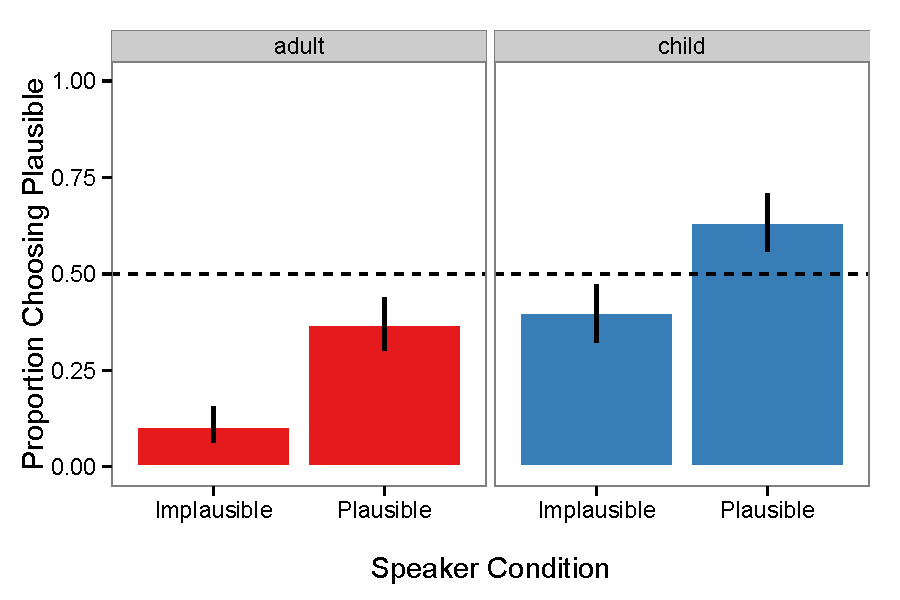
\includegraphics[width=5in]{figures/exp1_results.pdf}
    \caption{Experiment 1 test trial selections for both children and adults. In line with the predictions of a noisy channel model of language processing, both children and adults were more likely to correct the phonological error during Test trials when they were previously exposed to a Plausible Speaker. Bars show group-averaged proportion of plausible item selection at Test, error bars show 95\% confidence intervals computed by non-parametric bootstrap. The dashed line indicates chance performance.}%
   \label{fig:exp1_results}
\end{figure}

Did this exposure to a Plausible vs. Implausible speaker change participants' expectations on the ambiguous Test trials? Figure~\ref{fig:exp1_results} shows the proportion of both children and adults who selected the plausible referent at test in both conditions. As predicted, both groups were sensitive to the manipulation, selecting the plausible referent more often in the Plausible Speaker condition. While children were overall more likely to pick the plausible referent in both conditions, the effect size of the difference between conditions was nearly identical in adults and children, indicating equal adaptation to the Plausible vs. Implausible speaker ($d_{adult} =1.09$, $d_{child} = 1.10$). To confirm these findings formally, we again fit a mixed-effects regression predicting choice on Test trials from group (child vs. adult), condition (Plausible vs. Implausible Speaker), and their interaction. Both of the main effects were significant, but the interaction was not ($\beta_{child} = 1.96$,  $z = 3.33$, $p <.001$, $\beta_{Plausible Speaker} = 2.33$,  $z = 4.40$, $p <.001$,  $\beta_{child \: \cdot \: Plausible Speaker} = -1.01$,  $z = -1.53$, $p = .13$). Thus, children and adults, to the same degree, were more likely to select the plausible referent on ambiguous test trials when the speaker had previously referred to plausible referent on unambiguous Exposure trials.

When children and adults were exposed to a speaker who was likely to produce semantically implausible utterances (e.g. ``my cat has three little hammers''), they were more likely to interpret ambiguous utterances literally instead of error-correcting to a more semantically plausible alternative. Intriguingly, the size of this adaptation was nearly identical in both groups, suggesting that preschoolers are already adapting as rapidly as adults. Children were, however, more likely overall to pick the plausible referent during ambiguous test trials, suggesting that they generally rely more on their expectations than do adults. This finding is consonant with other evidence showing significantly more noise in children's perceptual systems \cite{neuman1983}.

\section{Experiment 2}

Experiment 2 replicates Experiment 1 in a larger sample of children across a broader age range, investigating the development of noisy channel processing.

\subsection{Method}

\subsubsection{Participants}

For Experiment 2, children were recruited from the floor of the San Jose Children's Discovery museum. An experimenter approached the child and parent and obtained informed consent before inviting both to enter a separate room in which an iPad and camera were set up. Data from a total of 146 children were collected, 6 of whom were excluded for $<50\%$ exposure to English. As before, children were recruited until at least 20 had been run in each condition for each of 3 age groups: 3, 4, and 5-year-olds. Children's ages were comparable within-groups across conditions, although gender varied more due to sampling (Plausible: 27 3-year-olds [16 girls, age: mean = 3.5, range = 3--3.93], 21 4-year-olds [7 girls, age: mean = 4.6, range = 4.22--4.97], 23 5-year-olds [19 girls, age: mean = 5.49, range = 5.01--5.95], Implausible: 21 3-year-olds [8 girls, age: mean = 3.49, range = 3.02--3.93], 28 4-year-olds [23 girls, age: mean = 4.51, range = 4--4.94], 20 5-year-olds [12 girls, age: mean = 5.48, range = 5.05--5.90].


\subsubsection{Stimuli, Design, \& Procedure}

Experiment 2 was an exact replication of Experiment 1.

\subsection{Results}

As in Experiment 1, we first establish that children understood the task, and encoded the differences between the Plausible and Implausible speakers on Exposure trials. First, we again ask whether children's behavior during the unambiguous exposure trials were sensitive to the speaker. We began by fitting a mixed-effects logistic regression for each age group separately, asking whether children's choices were sensitive to the speaker. In all 3 age groups, children were more likely to select the plausible referent when asked for it by the Plausible speaker (smallest $\beta_{3-years} = 1.43$, $z = 3.71$, $p < .001$). We then asked whether children's behavior changed over development. A mixed-effects model fit to all of the children's data showed main effects of both Age ($\beta = -.74$, $z = -4.18$, $p < .001$) and Speaker Plausibility ($\beta = -6.16$, $z = 1.81$, $p < .001$), and also an interaction between the two ($\beta = 2.12$, $z = 7.61$, $p < .001$). Thus, older children showed a greater sensitivity to the speaker on the unambiguous Exposure trials.

We next turned to the test trials, asking whether children's exposure to the Plausible vs. Implausible speakers changed their interpretation of the ambiguous utterances. 


Second, we again compared the conditions to each other, fitting a mixed-effects regression predicting choice on Exposure trials from noise level and speaker condition (Implausible, Plausible, Control). Compared to the Implausible Speaker condition, children exposed to the Plausible Speaker were more likely to pick the plausible referent on Exposure trials ($\beta_{Plausible} = 6.62$,  $z = 8.88$, $p <.001$). Children exposed to the Control speaker, who was identical to the Implausible speaker on Exposure trials, were not significantly different from those exposed to the Implausible speaker, as predicted ($\beta_{Control} = .36$,  $z = .83$, $p = .42$). Further, the model showed a marginal effect of Noise level ($\beta_{Noisy} = .86$,  $z = 1.74$, $p = .08$) and a significant interaction between Noise level and Speaker ($\beta_{Plausible \: \cdot \: Noisy} = -1.71$, $z= -2.15$, $p = .03$), indicating that the addition of noise moved children in both conditions closer to chance.


\section{Experiment 3}

Experiment 2 replicates Experiments 1 and 2 and tests a second prediction of noisy channel processing: As speech becomes noisier, children should rely more on their expectations.

\subsection{Method}

\subsubsection{Participants}

For Experiment 2, children were recruited from the floor of the San Jose Children's Discovery museum. An experimenter approached the child and parent and obtained informed consent before inviting both to enter a separate room in which an iPad and camera were set up. Data from a total of 114 children were collected, 1 of whom was excluded for $<50\%$ exposure to English and 2 of whom were excluded for parent-reported developmental disabilities. As before, children were recruited until at least 20 had been run in each condition. Children's ages and sexes were again comparable across conditions (Plausible, Noisy -- 26 children, 12 girls, age: mean = 4.98, min = 4.02, max = 5.94; Implausible, Noisy -- 24 children, 11 girls, age: mean = 5.01, min = 4.01, max = 5.92; Plausible, No Noise = 21 children, 8 girls, age: mean = 4.89, min = 4.1, max = 5.93; Implausible, No Noise --- 20 children, 12 girls, age: mean = 4.98, min = 4, max = 5.83; Control --- 20 children, 11 girls, age: mean = 4.96, min = 4.15, max = 5.91).
 
\subsubsection{Stimuli, Design, \& Procedure}

Stimuli were constructed as in Experiment 1 with a few small changes. First, one additional Test trial was added to increase power. Second, two versions of each acoustic recording were made. One was recorded in a sound-proof room by a female native English speaker. The second was constructed by convolving each recording with randomly generated Brown noise with an amplitude of .7. The first was used in the No Noise conditions, the second was used to replicate the two conditions from Experiment 1 as well as for the Control condition.

In addition, because all of the Test trials asked the listener to select the semantically implausible referent, it is possible that exposure to an Implausible speaker induced listeners to select the implausible referent at test generally, independent of their acoustic input.  In Experiment 2, we provide a Control condition in which the Implausible speaker from training asked for the semantically plausible referent at test. If children inferred from the unambiguous Exposure trials that the goal of the game was to pick the ``silly'' referent, they should have continued to select the implausible referent on Test trials. In contrast, if Exposure trials caused them to adjust the relative weights on acoustic information and linguistic expectations, they should instead have selected the plausible referent at test.

\subsection{Results}

As in Experiment 1, we first establish that children understood the task, and encoded the differences between the Plausible and Implausible speakers on Exposure trials. First, we ask whether children selected the plausible referent when it was asked for by the Plausible speaker, and selected the implausible referent when it was asked for by the Implausible speaker independent of noise level. We submitted performance for each condition and noise level separately to a mixed-effects logistic regression with random effects of subject and trial. As before, children were more likely than chance to choose the plausible referent in the Plausible condition, and less likely than chance to choose the plausible referent when the speaker asked for the implausible referent (smallest $\beta_{Control} = -.153$, $z = -4.32$, p < .001). 

Second, we again compared the conditions to each other, fitting a mixed-effects regression predicting choice on Exposure trials from noise level and speaker condition (Implausible, Plausible, Control). Compared to the Implausible Speaker condition, children exposed to the Plausible Speaker were more likely to pick the plausible referent on Exposure trials ($\beta_{Plausible} = 6.62$,  $z = 8.88$, $p <.001$). Children exposed to the Control speaker did not perform differently on Exposure trials from those exposed to the Implausible speaker, as predicted ($\beta_{Control} = .36$,  $z = .83$, $p = .42$). Further, the model showed a marginal effect of Noise level ($\beta_{Noisy} = .86$,  $z = 1.74$, $p = .08$) and a significant interaction between Noise level and Speaker ($\beta_{Plausible \: \cdot \: Noisy} = -1.71$, $z= -2.15$, $p = .03$), indicating that the addition of noise moved children in both conditions closer to chance.

\begin{figure}[t]
     \centering
     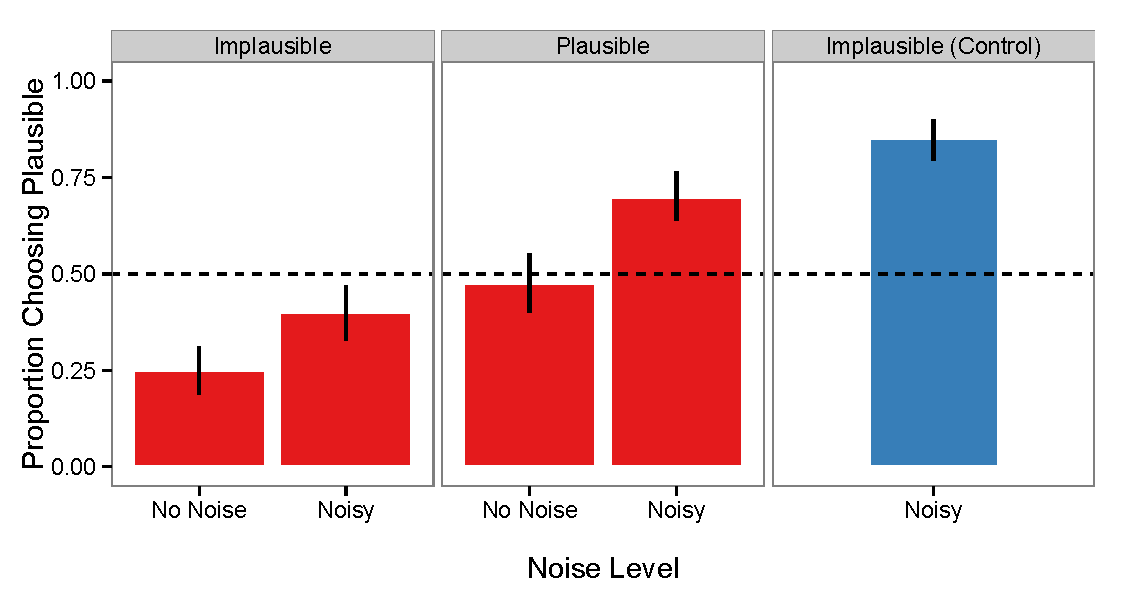
\includegraphics[width=5in]{figures/exp2_results.pdf}
    \caption{Experiment 2 Test trial responses. Replicating Experiment 1, children were more likely to correct the phonological error during Test trials when they were previously exposed to a Plausible speaker. In addition, in both conditions children were more likely to correct the error when the speech was noisier. Finally, when children were tested in a Control condition, in which a previously Implausible speaker referred to \emph{plausible} referents during ambiguous Test trials, they reliably selected the plausible referent. Together, these results show that children adaptively integrate both bottom-up acoustic information and top-down expectations about the speaker when processing language. Bars show group-averaged proportion of plausible item selection at test, error bars show 95\% confidence intervals computed by non-parametric bootstrap. The dashed line indicates chance performance.}%
   \label{fig:exp2_results}
\end{figure}

Did children integrate the noise level of the acoustic stimuli with speaker expectations on the ambiguous Test trials? Figure~\ref{fig:exp2_results} shows the proportion of trials on which children selected the plausible referent at test in both speaker and noise conditions. As predicted, children showed sensitivity to both speaker reliability and acoustic noise. Children selected the plausible referent at test, correcting the error in their acoustic input, more often when the speaker had said plausible things on Exposure trials (as in Experiment 1). In addition, regardless of Speaker plausibility, children selected the plausible referent more frequently when the acoustic input was noisy. To quantify this pattern, we again fit a mixed-effects regression predicting choice on test trials from Speaker type and Noise level as well as their interaction. As predicted, both main effects were significant ($\beta_{Plausible} = 1.96$,  $z = 3.20$, $p <.001$, $\beta_{Noisy} = .81$,  $z = 2.21$, $p = .03$), but their interaction was not ($\beta_{Plausible \: x \: Noisy} = .33$,  $z = .65$, $p = .51$).

Finally, one alternative explanation for the difference between Speaker conditions is that children simply followed their expectations at all times, e.g., that those exposed to the Implausible speaker chose ``silly'' responses regardless of the question. To test this alternative, we asked whether children who responded to an Implausible speaker on Exposure trials always chose the implausible referent on test trials even when the speaker referred to the \emph{plausible} referent (Implausible Control condition). A mixed-effects model estimating plausible referent selection on Test trials showed that compared to the Plausible speaker, children exposed to the Implausible speaker were less likely to pick the plausible referent ($\beta_{Implausible} = -1.57$,  $z = -4.14$, $p <.001$), but children in the Control condition were \emph{more} likely to select the plausible referent ($\beta_{Control} = 1.06$,  $z = 2.05$, $p = .04$). Thus, children who were asked for the plausible referent at Test selected it, even when the speaker had previously always referred to the implausible referent. This Control condition provides further evidence that children were attending to and responding to the acoustic input from the speaker on Test trials, integrating it with their prior expectations.


\section{General Discussion}

When we use language to communicate, we are doing more than processing the sounds we hear; we are trying to infer the speaker's intended meaning \cite{clark1996}. Because linguistic communication is inherently noisy, our expectations about what speakers are likely to say play an important role in resolving interpretive ambiguities \cite{grice1975, frank2012}. But how much should listeners rely on the acoustic signal and how much should they rely on their expectations? Ideal observer models of cue integration predict that each cue should be weighted in proportion to its reliability \cite{jacobs1999, ernst2002}. This prediction holds for adult listeners across levels in language processing from phonology to syntax \cite<e.g.,>{gibson2013, mcclelland2006, kleinschmidt2015}.Our experiments paper provide evidence that adaptive expectation-based language processing is already available to 4--5-year-old children. Not only do preschoolers combine their expectations about a speaker's likely utterance with the speech they are hearing, they flexibly re-weigh each as they develop stronger expectations about the speaker and as the speech signal changes in clarity.

Children adjusted their reliance on expectations as much as adults, but also relied relatively more on top-down expectations in general. Because of the greater noise inherent in children's perceptual processing systems, the same acoustic stimulus may effectively be less reliable for children than adults  \cite{neuman1983, lyons2011}. We can thus make a prediction about integration in atypical populations: Children with impaired acoustic processing should rely relatively more on their expectations, whereas children with impaired higher-level linguistic expectations (e.g., children with specific language impairment) should rely more on the acoustic signal.

% One puzzle of the broader literature on the development of language comprehension is that children appear to integrate information in an adult-like way in some language processing tasks but not others. A priori, we would predict that children's use of higher-level expectations should be relative to the reliability of their model of the relevant domain. Thus, children should---and do---integrate expectations when the relevant models are over speech sounds, speakers, or semantic plausibility \cite<e.g.,>{clark2009, creel2012, harris2012}. On the other hand, children tend to fail in cases where the relevant models include difficult linguistic content like quantifier semantics or complex syntactic constructions \cite<e.g.,>{trueswell1999, noveck2001}. 
% However, based on prior evidence that children's understanding of quantifiers is limited, as is their exposure to relative clauses, this is exactly the result a noisy channel framework for speech processing would predict  \cite{barner2011, montag2015}.

Noisy channel principles provide a framework for understanding language processing in both adults and children.
\section{Acknowledgments}

We thank Nicolette Castro, NIH NRSA F32HD075577 to DY, and a John Merck Scholars Fellowship to MCF.

\bibliographystyle{apacite}
\bibliography{noisy_kids}

\end{document}
